\chapter{Results}
% In this chapter, you should discuss the results you have obtained from your implementation.
% These can be correctness results, i.e whether the implementation behaved as expected, or numerical results that express runtime or energy measurements.

\section{Final program}
Our final program works as LED toggler combined with a clock. Each button is mapped to a single LED. When a button is pushed the coresponding LED is toggled. In addition a clock steadily decrements the LED value.

\section{Measurements}

\subsection{polling}
With our polling implementation as a baseline we measured about 4.9mA, regardless of button input. As expected, the polling method consumes a lot of energy since it constantly runs instructions whether they are needed or not. The result can be seen in figure \ref{fig:PerformancePolling}

\begin{figure}[ht]
 \centering
 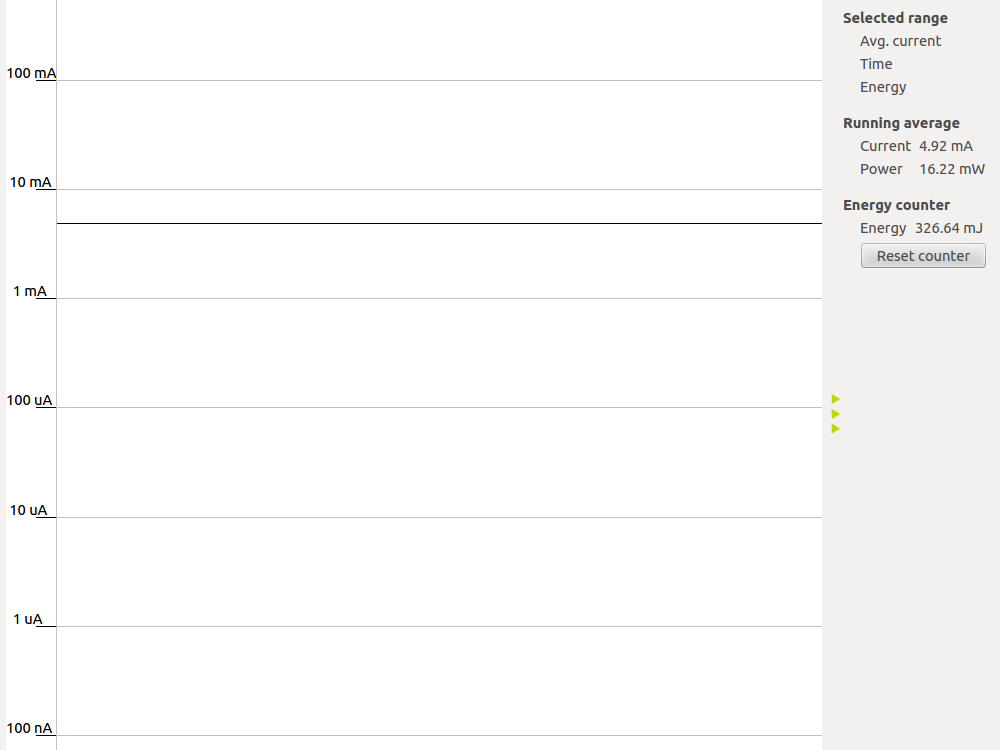
\includegraphics[width=\textwidth]{images/performance_with_polling.png}
 \caption{Energy consumption with polling}
 \label{fig:PerformancePolling}
\end{figure}

\subsection{interrupt}
Our wake on interrupt based program fared much better, averaging around 1.5$\mu$ A, and expending about 83$\mu$ A when a button was held down as seen in figure \ref{fig:PerformanceInterrupts}

\begin{figure}[ht]
 \centering
 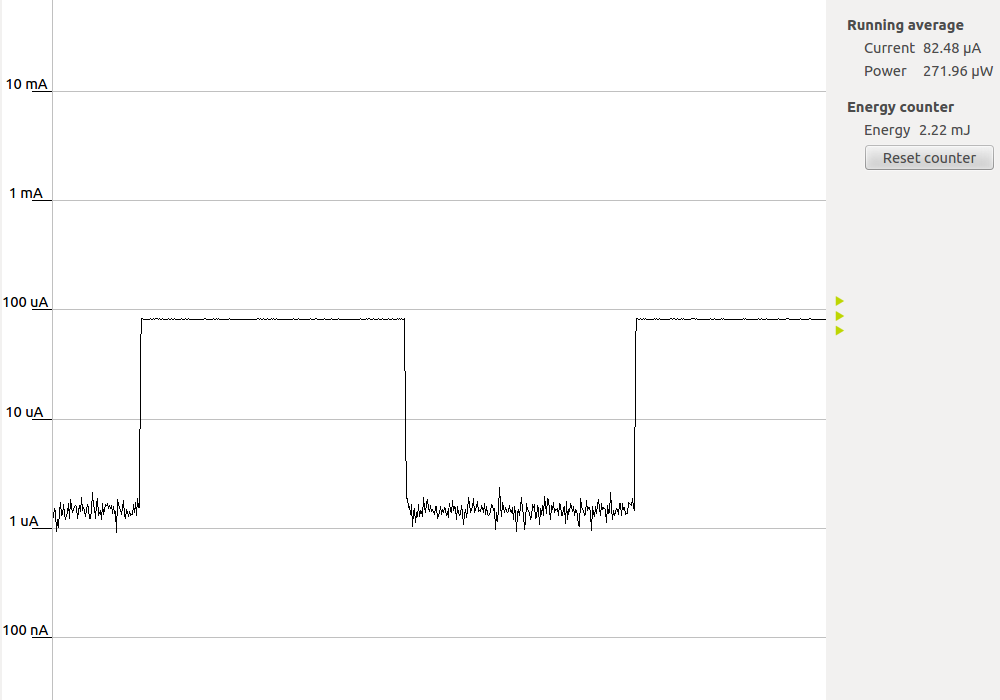
\includegraphics[width=\textwidth]{images/performance_with_interrputs.png}
 \caption{Energy consumption with interrputs}
 \label{fig:PerformanceInterrupts}
\end{figure}

\subsection{SRAM blocks}
In search of further improvement we powered down idle SRAM blocks to save more power, resulting in around 1$\mu$ A, a pretty substantial improvement from the simple interrupt based program. With a button held down however the difference was negligible as seen in figure \ref{fig:PerformanceSRAM}

\begin{figure}[ht]
 \centering
 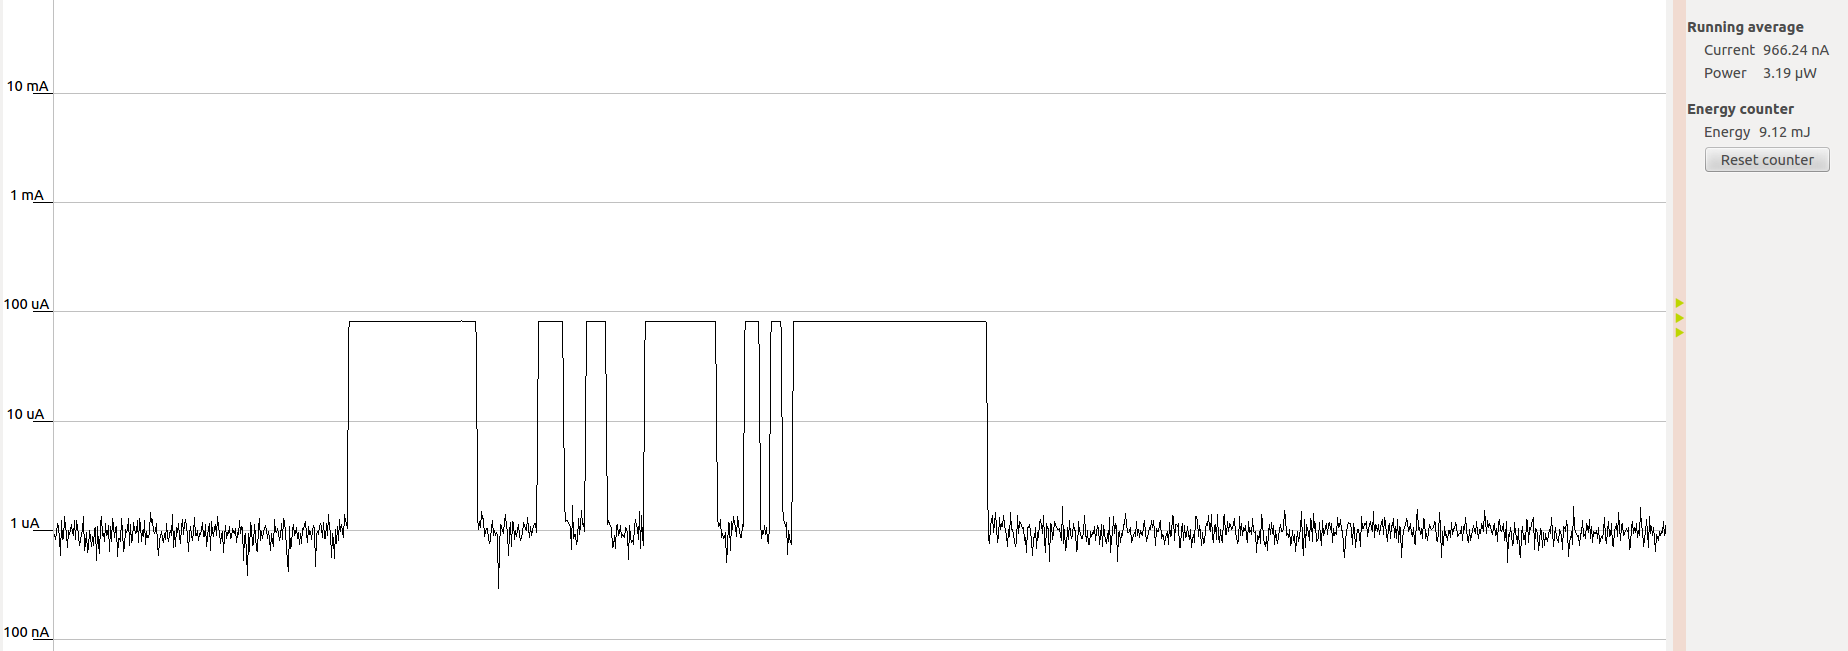
\includegraphics[width=\textwidth]{images/performance_interrupts_sram_idle.png}
 \caption{Energy consumption with interrputs, and SRAM blocks powered off}
 \label{fig:PerformanceSRAM}
\end{figure}

\subsection{Energy mode 3}
Turning off LFBCLK and setting LFACLK to use the ULFRCO set the device to energy mode 3, but we could measure no performance difference at all.

\subsection{}

\subsection{Noise}
In figure 4.2 and 4.3 a lot of noise can be seen when the board is in deep sleep. We could not find any specification about the measurment range and precision. It is unclear if the noise is caused by to low precision on the sensor, or if the other components on the board affects the sensor.